%%%%%%%%%%%%%%%%%%%%%%%%%%%%%%%%%%%
%This is the LaTeX ARTICLE template for RSC journals
%Copyright The Royal Society of Chemistry 2016
%%%%%%%%%%%%%%%%%%%%%%%%%%%%%%%%%%%

\documentclass[twoside,twocolumn,9pt]{article}
\usepackage{extsizes}
\usepackage[super,sort&compress,comma]{natbib} 
\usepackage[version=3]{mhchem}
\usepackage[left=1.5cm, right=1.5cm, top=1.785cm, bottom=2.0cm]{geometry}
\usepackage{balance}
\usepackage{mathptmx}
\usepackage{sectsty}
\usepackage{graphicx} 
\usepackage{lastpage}
\usepackage[format=plain,justification=justified,singlelinecheck=false,font={stretch=1.125,small,sf},labelfont=bf,labelsep=space]{caption}
\usepackage{float}
\usepackage{fancyhdr}
\usepackage{fnpos}
\usepackage[english]{babel}
\addto{\captionsenglish}{%
  \renewcommand{\refname}{Notes and references}
}
\usepackage{array}
\usepackage{droidsans}
\usepackage{charter}
\usepackage[T1]{fontenc}
\usepackage[usenames,dvipsnames]{xcolor}
\usepackage{setspace}
\usepackage[compact]{titlesec}
\usepackage{hyperref}
%%%Please don't disable any packages in the preamble, as this may cause the template to display incorrectly.%%%


\usepackage{epstopdf}%This line makes .eps figures into .pdf - please comment out if not required.

\definecolor{cream}{RGB}{222,217,201}

\usepackage{layout}

\begin{document}

\pagestyle{fancy}
\thispagestyle{plain}
\fancypagestyle{plain}{
%%%HEADER%%%
\renewcommand{\headrulewidth}{0pt}
}
%%%END OF HEADER


%%%PAGE SETUP - Please do not change any commands within this section%%%
\makeFNbottom
\makeatletter
\renewcommand\LARGE{\@setfontsize\LARGE{15pt}{17}}
\renewcommand\Large{\@setfontsize\Large{12pt}{14}}
\renewcommand\large{\@setfontsize\large{10pt}{12}}
\renewcommand\footnotesize{\@setfontsize\footnotesize{7pt}{10}}
\makeatother

\renewcommand{\thefootnote}{\fnsymbol{footnote}}
\renewcommand\footnoterule{\vspace*{1pt}% 
\color{cream}\hrule width 3.5in height 0.4pt \color{black}\vspace*{5pt}} 
\setcounter{secnumdepth}{5}

\makeatletter 
\renewcommand\@biblabel[1]{#1}            
\renewcommand\@makefntext[1]% 
{\noindent\makebox[0pt][r]{\@thefnmark\,}#1}
\makeatother 
\renewcommand{\figurename}{\small{Fig.}~}
\sectionfont{\sffamily\Large}
\subsectionfont{\normalsize}
\subsubsectionfont{\bf}
\setstretch{1.125} %In particular, please do not alter this line.
\setlength{\skip\footins}{0.8cm}
\setlength{\footnotesep}{0.25cm}
\setlength{\jot}{10pt}
\titlespacing*{\section}{0pt}{4pt}{4pt}
\titlespacing*{\subsection}{0pt}{15pt}{1pt}
%%%END OF PAGE SETUP%%%

%%%FOOTER%%%
\fancyfoot{}
\fancyfoot[LO,RE]{\vspace{-7.1pt}
\includegraphics[height=9pt]{auxiliary/rsc_template_head_foot/LF}}
\fancyfoot[CO]{\vspace{-7.1pt}\hspace{13.2cm}
\includegraphics{auxiliary/rsc_template_head_foot/RF}}
\fancyfoot[CE]{\vspace{-7.2pt}\hspace{-14.2cm}
\includegraphics{auxiliary/rsc_template_head_foot/RF}}
\fancyfoot[RO]{\footnotesize{\sffamily{1--\pageref{LastPage} ~\textbar  \hspace{2pt}\thepage}}}
\fancyfoot[LE]{\footnotesize{\sffamily{\thepage~\textbar\hspace{3.45cm} 1--\pageref{LastPage}}}}
\fancyhead{}
\renewcommand{\headrulewidth}{0pt} 
\renewcommand{\footrulewidth}{0pt}
\setlength{\arrayrulewidth}{1pt}
\setlength{\columnsep}{6.5mm}
\setlength\bibsep{1pt}
%%%END OF FOOTER%%%

%%%FIGURE SETUP - please do not change any commands within this section%%%
\makeatletter 
\newlength{\figrulesep} 
\setlength{\figrulesep}{0.5\textfloatsep} 

\newcommand{\topfigrule}{\vspace*{-1pt}% 
\noindent{\color{cream}\rule[-\figrulesep]{\columnwidth}{1.5pt}} }

\newcommand{\botfigrule}{\vspace*{-2pt}% 
\noindent{\color{cream}\rule[\figrulesep]{\columnwidth}{1.5pt}} }

\newcommand{\dblfigrule}{\vspace*{-1pt}% 
\noindent{\color{cream}\rule[-\figrulesep]{\textwidth}{1.5pt}} }

\makeatother
%%%END OF FIGURE SETUP%%%

%%%TITLE, AUTHORS AND ABSTRACT%%%
\twocolumn[
  \begin{@twocolumnfalse}
{
\includegraphics[height=30pt]{auxiliary/rsc_template_head_foot/journal_name}\hfill\raisebox{0pt}[0pt][0pt]{
\includegraphics[height=55pt]{auxiliary/rsc_template_head_foot/RSC_LOGO_CMYK}}\\[1ex]

\includegraphics[width=18.5cm]{auxiliary/rsc_template_head_foot/header_bar}}\par
\vspace{1em}
\sffamily
\begin{tabular}{m{4.5cm} p{13.5cm} }


\includegraphics{auxiliary/rsc_template_head_foot/DOI} & \noindent\LARGE{\textbf{Rapid technological progress in white light-emitting diodes and its sources in innovation and technology spillovers}} \\
\vspace{0.3cm} & \vspace{0.3cm} \\

 & \noindent\large{Michael Weinold \textit{$^{a b \ddag}$}, Sergey Kolesnikov,\textit{$^b$} and Laura Diaz Anadon\textit{$^{b}$}} \\

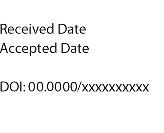
\includegraphics{auxiliary/rsc_template_head_foot/dates} & \noindent\normalsize{First commercial white light-emitting diodes (LEDs) were introduced to the market in 1996 . Since then, white LEDs have experienced major improvements in performance and decreases in cost, resulting in rapid market expansion of LED-based solid-state lighting (SSL), one of the key current solutions in global climate change mitigation efforts. Despite the significance of the technology, the extent and sources of these improvements have not been systematically investigated. Understanding what has driven rapid progress in LEDs can provide lessons for accelerating innovation in a broad range of other demand-side clean energy technologies for climate change mitigation. With this aim, we gather systematic evidence on cost and performance improvements in white LEDs from a literature review, interviews with experts in industry and academia, and results from our cost and performance modelling. We find that the overall efficiency of the highest performing warm white LED packages has improved from $\eta_L=5.8\%$ in 2003 to $\eta_L=38.7\%$ in 2020.  During the same period, we estimate that the cost of manufacturing low-power and mid-power LED packages at a U.S. location using state-of-the-art equipment has dropped from $1.1\$$ to $0.05\$$ (in 2020 USD) between 2003 and 2020, a $95.5\%$ decrease. We also show that technology spillovers—i.e., knowledge originating in other technologies—affected all performance dimensions of LEDs. They contributed no less than $8.5\%$ of the total efficiency improvements of devices and were responsible for $\sim 100\%$ of the improvements in consumer experience metrics. The increase in wafer size and manufacturing yield improvements were the primary causes of LED manufacturing cost reductions.}

\end{tabular}

 \end{@twocolumnfalse} \vspace{0.6cm}

  ]
%%%END OF TITLE, AUTHORS AND ABSTRACT%%%

%%%FONT SETUP - please do not change any commands within this section
\renewcommand*\rmdefault{bch}\normalfont\upshape
\rmfamily
\section*{}
\vspace{-1cm}


%%%FOOTNOTES%%%

\footnotetext{\textit{$^{a}$~ETH Zurich, Zurich, Switzerland. E-mail: michael.weinold@alumni.ethz.ch}}
\footnotetext{\textit{$^{b}$~Cambridge Centre for Environment, Energy and Natural Resource Governance, Department of Land Economy, University of Cambridge, Cambridge, United Kingdom. }}

%Please use \dag to cite the ESI in the main text of the article.
%If you article does not have ESI please remove the the \dag symbol from the title and the footnotetext below.
\footnotetext{\dag~Electronic Supplementary Information (ESI) available: [details of any supplementary information available should be included here]. See DOI: 00.0000/00000000.}
%additional addresses can be cited as above using the lower-case letters, c, d, e... If all authors are from the same address, no letter is required

\footnotetext{\ddag~Present address: Paul Scherrer Institut, Laboratory for Energy Analysis, Group for Technology Assessment, Switzerland.}


%%%END OF FOOTNOTES%%%

%%%MAIN TEXT%%%%

\section{Introduction}

A rapid reduction of global carbon dioxide emissions is urgently required in order to mitigate the effects of climate change \cite{Forster2019}. According to the United Nations, by the end of 2021, more than 130 countries have set or are considering setting a net zero emissions target by or around 2050 \cite{un2021climate}. The European Union, for example, has set a goal of net zero emissions by 2050—a goal it aims to meet with the help of the Green New Deal along other EU and national policies as part of the \textit{European Green Deal} \cite{eu2020green}. 

Achieving these ambitious and critically important targets will require both the deployment of new clean energy technologies, and the acceleration of innovation in existing supply-side \cite{sinn2012green} and demand-side technologies \cite{rgeVorsatz2009}. To ensure rapid adoption of these technologies, improvements in their costs, performance, and consumer experience are needed. This requires understanding how cost reductions and performance improvements can be achieved in these technologies \cite{Stephan2021}\cite{kolesnikov2020novel} \cite{Ziegler2021}.

There are a range of mechanisms that contribute to technological change in a technology over time, including targeted research and development (R\&D), economies of scale, learning by doing \cite{Arrow1971}, and economies of scope \cite{johansson2012global}\cite{national2016power}\cite{iea2020perspectives}. The role of these factors at different stages of the innovation life cycle \cite{grubler2012policies}, from research and technology development to demonstration, market formation and diffusion, is an area of active research \cite{Mowery1979} \cite{kavlak2018evaluating} \cite{kolesnikov2020novel} \cite{Ziegler2021}. Innovation is also driven by forces of supply and demand. Various \textit{"technology-push"} drivers reduce the costs of innovating, while \textit{"market-pull"} drivers increase the pay-offs from investing in innovation \cite{anadon2009policy}.

The stages and drivers of the innovation life-cycle for a particular technology play out within a broader innovation system \cite{grubler2012policies} \cite{Anadon2016}. Among these drivers, the role of knowledge transfer and technology spillovers in research and development of energy technologies is an understudied area \cite{Stephan2021}. While the exact definition of spillovers in literature depends on the context and the research question \cite{Liu2003}\cite{Nemet2012} we follow Stephan et al. \cite{Stephan2021} and consider knowledge to be external – thus a spillover –  if it has been developed for application in other technologies, sectors, or scientific disciplines. There is emerging evidence that understanding spillovers and the knowledge network outside a technology may be a fruitful approach to understand \cite{Pichler2020} and shape  \cite{Clark2016} \cite{ Stephan2021} \cite{Sun2021} the future evolution of technologies.  

Among demand-side technologies, the provision of lighting is a particularly important area  for climate change mitigation efforts, as it currently accounts for $15-19\%$ of global electricity consumption \cite{Zissis2016}\cite{doe_electricity}. It is also an area of rapid recent technological change: since the introduction of the first commercial white light-emitting diodes (LEDs) in 1996, lighting technology has experienced dramatic efficiency improvements. As shown in Figure 1, thanks to the introduction of LED-based solid-state lighting (SSL), the efficacy of lighting sources has increased by three orders of magnitude in just over 20 years, which is significantly faster than the historical progress observed in previous lighting technologies \cite{weinold2021quantifying}. For comparison, the highest performing light-emitting devices today reach efficacies of 220 lm/W \cite{lumistrips2021mid}, while an incandescent light bulb can only reach efficacies of up to 18 lm/W. Moreover, this rapid improvement in efficiency has been accompanied by a similarly impressive decrease in LED manufacturing costs and retail prices. During the same period, LED retail prices have fallen by two orders of magnitude, as shown in Figure 2.


\section{Conclusions}
Our study has analysed in a systematic and granular way the sources of dramatic cost reductions and efficiency improvements in white light-emitting diodes since their introduction to the market in 1996. We find that the total LED device efficiency increased from $5.8\%$ to $38.7\%$ between 2003 and 2020 has been predominantly driven by LED technology innovations that have affected all physical energy loss channels and corresponding device sub-efficiencies. We also find that among those innovations, at least nine were driven by technology originating in areas of science and technology outside LEDs and solid-state lighting—i.e., those nine innovations can be referred to as technology spillovers . These spillovers were responsible for $8.5\%$ of the total efficiency improvements and nearly $100\%$ of the improvements in consumer experience metrics. 

Our manufacturing cost model shows that a $95.5\%$ decrease in the cost of producing white classic-chip LEDs (from $1.11\$$ to $0.05\$$ in 2020 USD) between 2003 and 2020. While efficiency improvements have played an important role in these cost reductions, the largest components of such cost reductions have been driven by increases in the wafer size and yields across different manufacturing steps. In contrast with efficiency improvements, these increases were mainly a result of learning-by-doing and manufacturing equipment improvements rather than LED technology innovations or spillovers. 

Our analysis of the sources, mechanisms and enablers of the identified technology spillovers which were significant drivers of efficiency improvements, highlights the critical role played by a growing deep understanding of the physical, chemical and optical phenomena underlying the operation of LEDs, as well as materials science and technology and nanotechnology involved in the production of LEDs. Specifically, deep physical understanding of LED device efficiency loss channels enabled important breakthroughs and spillovers in LEDs and will enable further innovations to improve LED and SSL efficiency in the future, as expected by eminent experts in the field \cite{Weisbuch2020}. This suggests that additional research in these areas and a more deliberate search for spillovers may accelerate these expected future advances. Our findings on spillover enablers show that these efforts can be further supported or even accelerated by knowledge exchange events and long-term partnerships between academia and industry, dedicated mission-driven public R\&D funding, and freedom of search in academia. This reinforces arguments made against the dichotomy of basic research versus applied research \cite{narayanamurti2016cycles} \cite{narayanamurti2021genesis} and the calls for open, inclusive and flexible research cultures \cite{Stephan2021}.

There are various important avenues of future research that are opened up by our analysis. First, future work could expand the cost model by collecting and including data for a broader set of chip architectures and analyzing the impact of individual innovations and spillovers on costs as opposed to performance. Second, a deeper dive on the role of learning-by-doing is needed both in the cost and performance analysis to identify different types of learning by doing and how it came about. Third, building on the work on LED sub-efficiencies and physical limits, future efforts could focus on identifying priority areas for further efficiency improvements in LEDs and SSL in general. Finally, by comparing the drivers of innovation, technology spillovers, cost reductions and performance improvements at a granular level across different clean energy technologies, we can identify patterns or differences that would help us formulate recommendations for industry and policymakers aimed at accelerating further clean energy innovation for climate change mitigation. 

\section*{Conflicts of interest}
There are no conflicts to declare.

\section*{Acknowledgements}
This research is supported by a grant of the Alfred P. Sloan Foundation titled \href{http://web.archive.org/web/20200623065733/https://sloan.org/grant-detail/8567}{\textit{“What factors drive innovation in energy technologies? The role of technology spillovers and government investment”}}. Michael Weinold further gratefully acknowledges support by the \href{https://www.studienstiftung.ch/}{Swiss Study Foundation}. We would like to thank Venkatesh Narayanamurti, Gabriel Chan, Anna Goldstein, Didier Sornette, and participants of the SPIE West 2021 Conference and \href{https://www.ceenrg.landecon.cam.ac.uk/}{C-EENRG} Seminar Series of the University of Cambridge for many helpful discussions and feedback. We also express our deep gratitude to all interviewees for their willingness to participate in this study and their valuable contributions.

%%%END OF MAIN TEXT%%%

%The \balance command can be used to balance the columns on the final page if desired. It should be placed anywhere within the first column of the last page.

\balance

%If notes are included in your references you can change the title from 'References' to 'Notes and references' using the following command:
%\renewcommand\refname{Notes and references}

%%%REFERENCES%%%
\bibliography{auxiliary/rsc_style_files/bibliography_rsc}
\bibliographystyle{bibliography} %the RSC's .bst file

\end{document}
